% THIS DOCUMENT IS FOLLOWS THE VOLERE TEMPLATE BY Suzanne Robertson and James Robertson
% ONLY THE SECTION HEADINGS ARE PROVIDED
%
% Initial draft from https://github.com/Dieblich/volere
%
% Risks are removed because they are covered by the Hazard Analysis
\documentclass[12pt]{article}

\usepackage{booktabs}
\usepackage{tabularx}
\usepackage{graphicx}
\usepackage{float}
\usepackage{amsmath}

\usepackage{hyperref}
\hypersetup{
    bookmarks=true,         % show bookmarks bar?
      colorlinks=true,      % false: boxed links; true: colored links
    linkcolor=red,          % color of internal links (change box color with linkbordercolor)
    citecolor=green,        % color of links to bibliography
    filecolor=magenta,      % color of file links
    urlcolor=cyan           % color of external links
}

\newcommand{\lips}{\textit{Insert your content here.}}

%% Comments

\usepackage{color}

\newif\ifcomments\commentstrue %displays comments
%\newif\ifcomments\commentsfalse %so that comments do not display

\ifcomments
\newcommand{\authornote}[3]{\textcolor{#1}{[#3 ---#2]}}
\newcommand{\todo}[1]{\textcolor{red}{[TODO: #1]}}
\else
\newcommand{\authornote}[3]{}
\newcommand{\todo}[1]{}
\fi

\newcommand{\wss}[1]{\authornote{blue}{SS}{#1}} 
\newcommand{\plt}[1]{\authornote{magenta}{TPLT}{#1}} %For explanation of the template
\newcommand{\an}[1]{\authornote{cyan}{Author}{#1}}

%% Common Parts

\newcommand{\progname}{Housemates} % PUT YOUR PROGRAM NAME HERE
\newcommand{\authname}{Team \#9, Housemates
\\ Justin Dang - dangj15 
\\ Harris Hamid - hamidh1
\\ Fady Morcos - morcof2 
\\ Rizwan Ahsan - ahsanm7
\\ Sheikh Afsar - afsars} % AUTHOR NAMES                  

\usepackage{hyperref}
    \hypersetup{colorlinks=true, linkcolor=blue, citecolor=blue, filecolor=blue,
                urlcolor=blue, unicode=false}
    \urlstyle{same}
                                


\begin{document}

\title{Software Requirements Specification for \progname: Housemates App} 
\author{\authname}
\date{\today}
	
\maketitle

~\newpage

\pagenumbering{roman}

\tableofcontents

~\newpage

\section*{Revision History}

\begin{tabularx}{\textwidth}{p{3cm}p{2cm}X}
\toprule {\textbf{Date}} & {\textbf{Version}} & {\textbf{Notes}}\\
\midrule
October 6th 2023 & 0 & First Revision\\
\bottomrule
\end{tabularx}

~\\

~\newpage
\section{Purpose of the Project}
\subsection{User Business}

With the ongoing affordable housing shortage in Canada many people have been forced to find roommates in order to have a place to live in. This is especially common at universities like McMaster where its extremely common to have housemates while in student housing. While having roommates may help ease financial pressures it can lead to a lot of stress in dealing with them. These stresses can include things like dealing with splitting household tasks and grocery costs. An application that helps deal with these common stresses in the roommate life would make it more convenient  for the housemates to live together and overall simplify their lives.

\subsection{Goals of the Project}

\begin{center}
\begin{tabular}{|p{6cm}|p{6cm}|}
\hline
\textbf{Goals} & \textbf{Importance}\\
\hline The application will have a straightforward and user-friendly interface that is simple to use for all users, regardless of technical ability. & This allows first time users to be interested in our product and a good experience with the overall product. \\
\hline
The application will simplify household task management through a task management system. & This allows streamlining the allocation of chores which in return will reduce conflicts and misunderstandings between housemates. \\
\hline
The application will streamline expense sharing through a cost management system. & This makes it possible for roommates to monitor their expenditure and prevent overspending. Additionally, it encourages each person to make a fair financial contribution. \\
\hline
The application will have a scheduling system that will allow for users to schedule quiet hours & This allows users to focus on their work, sleep, or studies without any interruption. \\
\hline
The application will have a calendar to see scheduled events & This allows users to coordinate their schedules and help them in managing their time in a better way. \\
\hline
\end{tabular}
\end{center}

\section{Stakeholders}
\subsection{Client}

N/A

\subsection{Customer}

\begin{itemize}
    \item People with housemates: People with housemates are the primary stakeholders of this application. They can use the application to better simplify life with housemates. As such they will have the greatest influence out of the stakeholders on the requirements of the application during the development process.
\end{itemize}

\subsection{Other Stakeholders}

\begin{itemize}
  \item Landlords / Property Manager / Housing Association: Landlords would be a secondary stakeholder for the application. Landlords might be interested in using an application like this for their tenants so that they will better be able to communicate with them with respects to household tasks that are required. As such, they might play a minor role on determining the requirements of the application during the design process.
  \item Families: Families can also benefit from the app to have a centralized place for all household matters. They can distribute chores evenly and keep track of bills. It promotes talking openly and encourages users to be more responsible about household duties and bills.
\end{itemize}

\subsection{Hands-On Users of the Project}

\begin{itemize}
    \item People with housemates
    \item Landlords / Property Manager / Housing Association
    \item Families
\end{itemize}

\subsection{Personas}
Andrew is a student at McMaster University. He lives off-campus in student housing with four other housemates. He and his roommates have to buy groceries and supplies for the house. They also have to do various household chores and pay for utilities and internet. Sometimes Andrew and his roommates have trouble communicating with one another on this. Additionally, Andrew gets annoyed when his roommates decide to have a party the day before Andrew has an exam.

\subsection{Priorities Assigned to Users}

The primary stakeholders for this project are people with housemates and as such they will have the highest priority during the development process. The other stakeholders will be considered during the development process, but overall will have a lower priority.

\subsection{User Participation}

During the development process we plan to test the application with the stakeholders described above. Their feedback will help improve the application to better fit their needs.

\subsection{Maintenance Users and Service Technicians}

During the development of this project the project will be maintained by the development team.

\section{Mandated Constraints}
\subsection{Solution Constraints}

N/A

\subsection{Implementation Environment of the Current System}

The expected environment for this application will be mobile devices (Android, iOS), providing a user-friendly and intuitive application that is really simple to use. With goals of expanding to web application, so that we can cater to a much diverse user base using computers with Windows, Max or Linux and web browsers such as Chrome, Edge, Firefox, etc. Users would then have the convenience to access the solution/product on any device they want that suits their needs. 

\subsection{Partner or Collaborative Applications}

N/A

\subsection{Off-the-Shelf Software}

N/A

\subsection{Anticipated Workplace Environment}
The anticipated workplace environment for this application is in users' homes since this application deals with roommates. However, as this app is on mobile devices there could be a wide variety of places where this application could be used.

\subsection{Schedule Constraints}
This project is being developed from September 2023 - April 2024.
\subsection{Budget Constraints}
This project has a budget constraint of \$750.
\subsection{Enterprise Constraints}
N/A

\section{Naming Conventions and Terminology}
\subsection{Glossary of All Terms, Including Acronyms, Used by Stakeholders
involved in the Project}
\begin{itemize}
    \item Android: A mobile operating system designed for mobile devices.
    \item Google Play Store: The most common app store on Android. 
\end{itemize}

\section{Assumptions}
% \subsection{Relevant Facts}
% \lips
% \subsection{Business Rules}
% N/A
\begin{itemize}
    \item The users of this application are expected to have a basic understanding of how to use mobile devices with a touchscreen.
\end{itemize}

% \section{The Scope of the Work}
% \subsection{The Current Situation}
% \lips
% \subsection{The Context of the Work}
% \lips
% \subsection{Work Partitioning}
% \lips
% \subsection{Specifying a Business Use Case (BUC)}
% \lips
% Don't think we neeed this part yet

% \section{Business Data Model and Data Dictionary}
% \subsection{Business Data Model}
% \lips
% % \subsection{Data Dictionary}
% % \lips
% % Dont think we need this part yet

\section{Scope}
\subsection{Product Context}
The following diagram depicts the main application interacting with external systems and users and the relation between them in terms of data flow.
\begin{figure}[H]
    \centering
	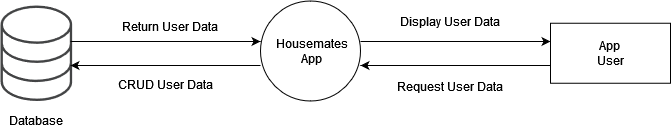
\includegraphics[width=15cm]{ContextDiagram.png}
	\caption{Context Diagram}
 \label{}
\end{figure}
\subsection{Product Use Case Diagram}
\begin{figure}[H]
    \centering
	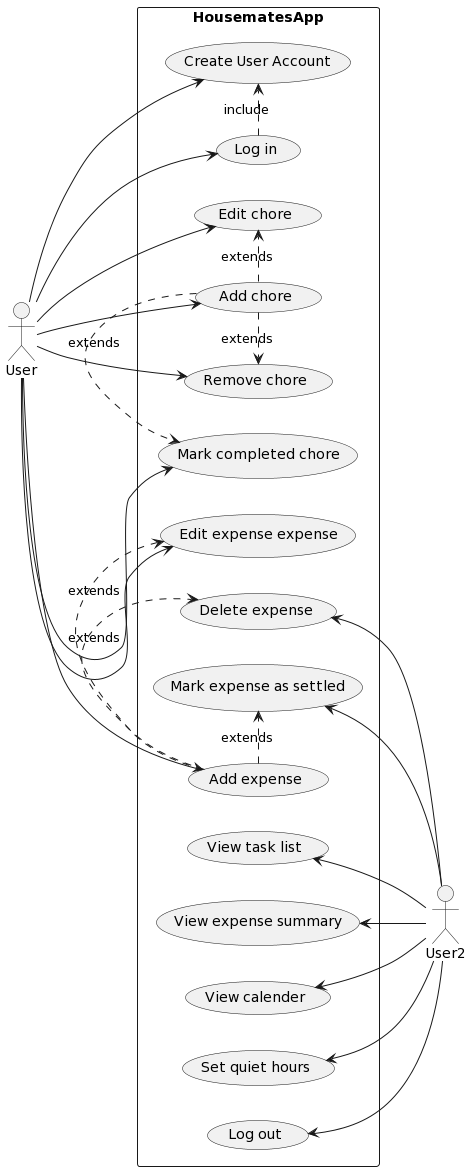
\includegraphics[width=6.5cm]{UseCase.png}
	\caption{Usecase Diagram}
 \label{}
\end{figure}
\subsection{Individual Product Use Cases (PUC's)}
\begin{itemize}
    \item[PUC1:]
        \begin{itemize}
            \item \textbf{\textit{Title}: Create user account}
            \item \textit{Precondition}: User does not have existing account.
            \item \textit{Trigger}: User selects option to create new account.
            \item \textit{Description}:Allows user to provide necessary information (such as name, email, password) to create a new account within the system.
    \end{itemize}

    \item[PUC2:]
        \begin{itemize}
            \item \textbf{\textit{Title}: Log in}
            \item \textit{Precondition}: User has an existing account.
            \item \textit{Trigger}: User enters their information and selects the log in option.
            \item \textit{Description}: Allows user to authenticate and access their existing account.
    \end{itemize}

    \item[PUC3:]
        \begin{itemize}
            \item \textbf{\textit{Title}: Add household chores}
            \item \textit{Precondition}: User is logged in and has housemates added.
            \item \textit{Trigger}: User selects the option to add a new household chore.
            \item \textit{Description}: Enables users to create a new household chore with details like name, description, frequency and assign it.
    \end{itemize}

    \item[PUC4:]
        \begin{itemize}
            \item \textbf{\textit{Title}: Edit household chores}
            \item \textit{Precondition}: User is logged in and has existing household chore.
            \item \textit{Trigger}: User selects the option to edit an existing household chore.
            \item \textit{Description}: Allows users to modify details of an existing household chore, such as its name, description, frequency and assignee.
    \end{itemize}

    \item[PUC5:]
        \begin{itemize}
            \item \textbf{\textit{Title}: Remove household chores}
            \item \textit{Precondition}: User is logged in and has existing household chore.
            \item \textit{Trigger}: User selects the option to delete an existing household chore.
            \item \textit{Description}: Allows users to remove a household chore that is no longer required.
    \end{itemize}

    \item[PUC6:]
        \begin{itemize}
            \item \textbf{\textit{Title}: Marking completion of household chores}
            \item \textit{Precondition}: User is logged in and has existing household chore.
            \item \textit{Trigger}: User selects the option to mark a household chore as completed.
            \item \textit{Description}: Allows users to mark off a specific household chore and track that it has been successfully completed.
    \end{itemize}

    \item[PUC7:]
        \begin{itemize}
            \item \textbf{\textit{Title}: Add expense}
            \item \textit{Precondition}: User is logged in.
            \item \textit{Trigger}: User selects the option to add a new household expense.
            \item \textit{Description}: Enables users to record a new expense between all or specific housemates, including details like item name, cost, date of purchase, etc.
    \end{itemize}

    \item[PUC8:]
        \begin{itemize}
            \item \textbf{\textit{Title}: Edit expense}
            \item \textit{Precondition}: User is logged in and has existing existing expense.
            \item \textit{Trigger}: User selects the option to edit an existing expense.
            \item \textit{Description}: Allows users to modify details of an existing expense.
    \end{itemize}

    \item[PUC9:]
        \begin{itemize}
            \item \textbf{\textit{Title}: Delete expense}
            \item \textit{Precondition}: User is logged in and has existing expense.
            \item \textit{Trigger}: User selects the option to delete an existing expense.
            \item \textit{Description}: Enables users to remove an expense that is no longer relevant or was added by mistake.
    \end{itemize}

    \item[PUC10:]
        \begin{itemize}
            \item \textbf{\textit{Title}: Mark expense as settled}
            \item \textit{Precondition}: User is logged in and has existing household chore.
            \item \textit{Trigger}: User selects the option to mark a household chore as completed.
            \item \textit{Description}: Allows users to mark off a specific household chore and track that it has been successfully completed.
    \end{itemize}

    \item[PUC11:]
        \begin{itemize}
            \item \textbf{\textit{Title}: View task list}
            \item \textit{Precondition}: User is logged in and has existing tasks/chores.
            \item \textit{Trigger}: User selects the option to view the task list.
            \item \textit{Description}: Displays a list of all current tasks for the user's household.
    \end{itemize}

    \item[PUC12:]
        \begin{itemize}
            \item \textbf{\textit{Title}: View expense summary}
            \item \textit{Precondition}: User is logged in and has existing expenses.
            \item \textit{Trigger}: User selects the option to view the expense summary.
            \item \textit{Description}: Displays an overview of shared expenses and individual contributions.
    \end{itemize}

    \item[PUC13:]
        \begin{itemize}
            \item \textbf{\textit{Title}: View calendar}
            \item \textit{Precondition}: User is logged in.
            \item \textit{Trigger}: User selects the option to view the calendar.
            \item \textit{Description}: Displays a calendar with scheduled events, tasks, and quiet hours.
    \end{itemize}

    \item[PUC14:]
        \begin{itemize}
            \item \textbf{\textit{Title}: Set quiet hours}
            \item \textit{Precondition}: User is logged in and has housemates added.
            \item \textit{Trigger}: User selects the option to set quiet hours.
            \item \textit{Description}: Allows users to define specific time periods for quiet hours in the living space.
    \end{itemize}

    \item[PUC15:]
        \begin{itemize}
            \item \textbf{\textit{Title}: Log out}
            \item \textit{Precondition}: User is logged.
            \item \textit{Trigger}: User selects the option to log out.
            \item \textit{Description}: Allows a logged-in user to securely log out of their account, ending their current session.
    \end{itemize}


\end{itemize}



\section{Functional Requirements}
\subsection{Task Management System}
\noindent \begin{itemize}
    \item[TM1:] 
    \begin{itemize}
        \item \textit{Description}: Housemates app will have a tile like interface where user can select tasks icon as one of the options to then navigate to the task management page
        \item \textit{Rationale}: This is to be able to navigate to the task management page of the app instead of utilizing one of the other features
        \item \textit{Fit Criterion}: User can tap on the tasks icon and reach the page for task management
    \end{itemize}
    \item[TM2:] 
    \begin{itemize}
        \item \textit{Description}: The task management page will have a list-like interface presenting to the user their chores that they need to completed highlighted amongst other roommates tasks.
        \item \textit{Rationale}: This is to be able to clearly view the tasks which the user must complete
        \item \textit{Fit Criterion}: User can clearly understand which chores they need to complete
    \end{itemize}
    \item[TM3:] 
    \begin{itemize}
    \item \textit{Description}: In the task management page, users are able to create new tasks/chores and add them to the task management page.
    \item \textit{Rationale}: Users need to be able to add new chores/tasks as needed.
    \item \textit{Fit Criterion}: 
    \begin{enumerate}
        \item Users are able to access a "Create New Task" button on the task management page.
        \item A task creation form is shown after the user presses on this button.
        \item The form fields have a spot for task name, due date, and roommate assignment (if applicable).
        \item After the user filling out the form and presses the "Create," button the new task now appears in the list of tasks.
    \end{enumerate}
    \end{itemize}
    \item[TM4:]
    \begin{itemize}
    \item \textit{Description}: In the task management page, users can assign tasks to roommates if the chore is shared.
    \item \textit{Rationale}: This feature enables users to divide tasks among roommates.
    \item \textit{Fit Criterion}: 
    \begin{enumerate}
        \item Users can select a task from the list by pressing on the task.
        \item Users can assign the task to other roommates from their list of roommates.
    \end{enumerate}
    \end{itemize}
    \item[TM5:]
    \begin{itemize}
    \item \textit{Description}: In the task management page, users can mark tasks as completed.
    \item \textit{Rationale}: Users need to be allowed to track the progress of tasks and mark them as completed when they are done.
    \item \textit{Fit Criterion}: 
    \begin{enumerate}
        \item Users is able to select a task from the list.
        \item Users is able to mark the task as completed.
        \item The user can see that the task is marked as completed on the task management page.
    \end{enumerate}
    \end{itemize}
    
\end{itemize}
\subsection{Bill Management System}
\noindent \begin{itemize}
    \item[BM1:] 
    \begin{itemize}
        \item \textit{Description}: Users are able to create a new bill.
        \item \textit{Rationale}: This requirement allows users to create new bills as needed.
        \item \textit{Fit Criterion}: Users can add new bills by providing bill name, amount paid, category, due date, etc
    \end{itemize}
    \item[BM2:] 
    \begin{itemize}
        \item \textit{Description}: Users are able to assign bill to a housemate and split it between them.
        \item \textit{Rationale}: This functionality will allow users to keep track of bill splitting easily.
        \item \textit{Fit Criterion}: 
        \begin{enumerate}
            \item The bill amount is correctly split between the housemates.
            \item The total bill amount is shown on the screen and the amount required to pay by each housemate is displayed correctly.
        \end{enumerate}
    \end{itemize}
    \item[BM3:] 
    \begin{itemize}
        \item \textit{Description}: Users are able to modify already inputted bill details 
        \item \textit{Rationale}: This requirement allows users to modify any information on the bill for any correction or changes.
        \item \textit{Fit Criterion}: Users can view and edit any bill on the page and the changes are saved and reflected correctly on the system.
    \end{itemize}
    \item[BM4:] 
    \begin{itemize}
        \item \textit{Description}: Users are able to categorize the bills.
        \item \textit{Rationale}: This requirements makes it easier for users to differentiate and organize their expenses.
        \item \textit{Fit Criterion}: Users can assign bills to any specific categories such as utility, rent, groceries, etc
    \end{itemize}
    \item[BM5:] 
    \begin{itemize}
        \item \textit{Description}: Users are able to keep track of which bills have been paid off.
        \item \textit{Rationale}: This requirement will allow users to keep track of their payments.
        \item \textit{Fit Criterion}: 
        \begin{enumerate}
            \item Users can mark any bill they paid off and the system keeps a record of the history.
            \item When a bill is paid off, the included housemates are provided with a notification.
        \end{enumerate}
    \end{itemize}
    \item[BM6:] 
    \begin{itemize}
        \item \textit{Description}: Users are able to attach bill receipts or relevant information as pictures.
        \item \textit{Rationale}: This functionality will allow users to share any receipts or relevant document if they see fit.
        \item \textit{Fit Criterion}: Users are able to upload files and images to the specific bill and the app updates it properly.
    \end{itemize}
    \item[BM7:] 
    \begin{itemize}
        \item \textit{Description}: Users are able to search for any specific bill.
        \item \textit{Rationale}: This will allow users to navigate and search for any specific bill allowing them to save time.
        \item \textit{Fit Criterion}: Users are able to search bills by their name, category, etc
    \end{itemize}
\end{itemize}



\subsection{Scheduling System}
\noindent \begin{itemize}
    \item[SS1: ]
\begin{itemize}
    \item \textit{Description}: Roommates are able to navigate to the scheduling page to use the scheduling feature by tapping the scheduling icon from the home interface to get to the scheduling page.
    \item \textit{Rationale}: This functionality allows the app to be divided into sections depending on feature for clear usability
    \item \textit{Fit Criterion}: Users can clearly distinguish from which section they want to utilize.
\end{itemize}
    
    \item[SS2: ]
\begin{itemize}
    \item \textit{Description}: Roommates are able to create new events and schedule them within the scheduling feature.
    \item \textit{Rationale}: This functionality allows roommates to plan and coordinate activities efficiently.
    \item \textit{Fit Criterion}:
    \begin{enumerate}
        \item Users can tap on "Create New Event"  within the Housemates app on the scheduling page.
        \item Users are able fill out an event creation form with details such as event name, date, time, duration, and a brief description.
        \item After creation, the new event is listed in the scheduling feature and is able to be seen be all the users/roommates.
    \end{enumerate}
\end{itemize}

\item[SS3: ]
\begin{itemize}
    \item \textit{Description}: Users can view all the events scheduled by other roommates on their calendar within the scheduling feature.
    \item \textit{Rationale}: Event visibility ensures that all roommates are aware of shared activities and can plan accordingly.
    \item \textit{Fit Criterion}: Users can clearly see and distinguish between their personal events and shared roommate events on the calendar.
\end{itemize}
    
\end{itemize}
\subsection{Account System}
\noindent \begin{itemize}
    \item[AS1:] 
    \begin{itemize}
        \item \textit{Description}: Users can create new account by providing their personal information.
        \item \textit{Rationale}: This requirement is essential to allow new users to use the product and personalize their experience within the app.
        \item \textit{Fit Criterion}: The system should allow successful registration of users when they provide valid information
    \end{itemize}
    \item[AS2:] 
    \begin{itemize}
        \item \textit{Description}: Users are able to log in to the system by providing their email address/username and password.
        \item \textit{Rationale}: This requirement ensures that only authorized users are able to access their accounts and the features available in the app.
        \item \textit{Fit Criterion}: 
        \begin{enumerate}
            \item Users will be able to successfully log in to the app provided they give valid credentials
            \item Users will be unable to log in if they provide invalid credentials and appropriate error message will be shown.
        \end{enumerate}
    \end{itemize}
    \item[AS3:] 
    \begin{itemize}
        \item \textit{Description}: Users are able to update their profile information.
        \item \textit{Rationale}: This requirement will allow user to change their information when they see fit.
        \item \textit{Fit Criterion}: Changes made in the profile section should be updated and reflected properly in the app.
    \end{itemize}
    \item[AS4:] 
    \begin{itemize}
        \item \textit{Description}: Users are able to remove their account from the system.
        \item \textit{Rationale}: Users should be given the option to have control of their own account.
        \item \textit{Fit Criterion}: 
        \begin{enumerate}
            \item Users can temporarily deactivate their account and reactivate them.
            \item Users can permanently delete their account.
        \end{enumerate}
    \end{itemize}
    \item[AS5:] 
    \begin{itemize}
        \item \textit{Description}: Users are able to recover their account in case of forgetting their log in information
        \item \textit{Rationale}: This requirement allows users a way to recover their account and seek support.
        \item \textit{Fit Criterion}: Users are able to click a "Forgot Password" button if they forgot their password which sends an email to their provided email address.
    \end{itemize}
\end{itemize}
\subsection{Formal Specification of Cost Management System}

A critical aspect of this project involves calculating expenses associated to every housemate. In order to represent all costs and expense associated to every housemate in an accurate and timely fashion, we will formally represent this system using Module Interface Specification. \\

Let:

\begin{itemize}
    \item $I$ be the set of all individual items or bills.
    \item $U$ be the set of all users. (Housemates/Roommates etc)
    \item $C$ be the cost associated with each item.
    \item $S$ be a function that maps an item to its sharers.
    \item $P$ be a function that maps an item to its payment division.
\end{itemize}

\subsubsection*{Individual Costs}

For each item $i$ in $I$, there is a cost $c$ associated with it. Formally:

\[
C: I \rightarrow R^+
\]

This function $C$ maps every item $i$ to its positive cost $c$.

\subsubsection*{Sharers of Costs}

For each item $i$, there's a subset of users $U_i \subseteq U$ who share its cost. The function $S$ determines which users are responsible for which items:

\[
S: I \rightarrow 2^U
\]

Here, $2^U$ represents the power set of $U$, denoting all possible subsets of users. Not all users necessarily owe an amount.

\subsubsection*{Payment Division}

The function $P$ assigns a portion of the item's cost to each user:

\[
P: I \times U \rightarrow R^+
\]

This means for each item $i$ and user $u$ in $U_i$, $P(i, u)$ returns the amount $u$ owes for $i$. For users not in $U_i$, $P(i, u) = 0$.

\subsubsection*{Constraints}

\subsubsection*{Total Payment}

The total amount paid by all users for an item must equal the cost of that item:

\[
\forall i \in I: \sum_{u \in U} P(i, u) = C(i)
\]

\subsubsection*{Non-negative Payment}

No user can owe a negative amount:

\[
\forall i \in I, \forall u \in U: P(i, u) \geq 0
\]

\subsubsection*{Overall User Expense}

The total amount owed by a user for all items is:

\[
\text{Expense}: U \rightarrow R^+
\]

\[
\text{Expense}(u) = \sum_{i \in I} P(i, u)
\]


\section{Look and Feel Requirements}
\subsection{Appearance Requirements}
\noindent \begin{itemize}
    \item[LF-A1:] 
    \begin{itemize}
        \item \textit{Description}: The application should have a modern minimalist user interface.
        \item \textit{Rationale}: A minimalist user interface design will allow users to intuitively use the application.
        \item \textit{Fit Criterion}: The interface follows the minimalist design principles in \href{https://m3.material.io/foundations}{Google's material design guidelines}. 
    \end{itemize}
\end{itemize}

\subsection{Style Requirements}

N/A

% \noindent \begin{itemize}
%     \item[LF-S1:] 
%     \begin{itemize}
%         \item \textit{Description}: 
%         \item \textit{Rationale}: 
%         \item \textit{Fit Criterion}: 
%     \end{itemize}
% \end{itemize}

\section{Usability and Humanity Requirements}
\subsection{Ease of Use Requirements}

\noindent \begin{itemize}
    \item[UH-E1:] 
    \begin{itemize}
        \item \textit{Description}: The application should be easy to navigate.
        \item \textit{Rationale}: Users of the application should able to reach the main features of the application clearly.
        \item \textit{Fit Criterion}: Users of the application should be able to reach the main features of the application within 5 clicks/taps.
    \end{itemize}
\end{itemize}

\subsection{Personalization and Internationalization Requirements}
\noindent \begin{itemize}
    \item[UH-P1:] 
    \begin{itemize}
        \item \textit{Description}: The application will use Canadian English as its primary language.
        \item \textit{Rationale}: Most of the target audience of the application speak English.
        \item \textit{Fit Criterion}: The application uses Canadian English when released.
    \end{itemize}
\end{itemize}

\subsection{Learning Requirements}
\noindent \begin{itemize}
    \item[UH-L1:] 
    \begin{itemize}
        \item \textit{Description}: Users of the application should be able to quickly learn how to use it.
        \item \textit{Rationale}: The application should be easy to learn.
        \item \textit{Fit Criterion}: During testing a user should able to use all of the features of the application within the first 30 minutes of first opening the application.
    \end{itemize}
\end{itemize}
\subsection{Understandability and Politeness Requirements}

N/A

% \noindent \begin{itemize}
%     \item[UH-UP1:] 
%         \begin{itemize}
%            \item \textit{Description}: 
%             \item \textit{Rationale}: 
%             \item \textit{Fit Criterion}: 
%         \end{itemize}
% \end{itemize}
\subsection{Accessibility Requirements}
\noindent \begin{itemize}
    \item[UH-A1:] 
        \begin{itemize}
            \item \textit{Description}: The application should be usable by partially sighted users.
            \item \textit{Rationale}: Accessibility accommodations will allow the app to reach a larger target audience.
            \item \textit{Fit Criterion}: The application uses the various \href{https://support.google.com/accessibility/android/answer/6006564?hl=en}{android accessibility features.}
        \end{itemize}
\end{itemize}

\section{Performance Requirements}
\subsection{Speed and Latency Requirements}
\noindent \begin{itemize}
    \item[P-SL1:] 
        \begin{itemize}
            \item \textit{Description}: The application should respond to user interactions quickly.
            \item \textit{Rationale}: Users should feel the app is responsive.
            \item \textit{Fit Criterion}: The application should respond to user input within 0.5 seconds.
        \end{itemize}
\end{itemize}
\subsection{Safety-Critical Requirements}

N/A

% \noindent \begin{itemize}
%     \item[P-SC1:] 
%         \begin{itemize}
%            \item \textit{Description}: 
%             \item \textit{Rationale}: 
%             \item \textit{Fit Criterion}: 
%         \end{itemize}
% \end{itemize}
\subsection{Precision or Accuracy Requirements}
\noindent \begin{itemize}
    \item[P-PA1:] 
        \begin{itemize}
            \item \textit{Description}: All monetary information (e.g. bill amounts) will be accurate to two decimal places. 
            \item \textit{Rationale}: Information from cost-splitting system should be accurate.
            \item \textit{Fit Criterion}: During testing costs will be correctly rounded to two decimal places.
        \end{itemize}
\end{itemize}
\subsection{Robustness or Fault-Tolerance Requirements}
\noindent \begin{itemize}
    \item[P-RFT1:] 
        \begin{itemize}
            \item \textit{Description}: The application should continue to operate locally if it loses connection to the server.
            \item \textit{Rationale}: Users may temporarily lose connection to the application servers during use.
            \item \textit{Fit Criterion}: The application should continue to function for 10 minutes after losing connection to application servers. Additionally it should function as normal when connection is resumed.
        \end{itemize}
\end{itemize}
\subsection{Capacity Requirements}
\noindent \begin{itemize}
    \item[P-C1:] 
        \begin{itemize}
            \item \textit{Description}: The application should be able to handle 100 simultaneous users.
            \item \textit{Rationale}: The application should be handle a lot of users using it at the same time.
            \item \textit{Fit Criterion}: During testing the application should handle 100 simultaneous users.
        \end{itemize}
\end{itemize}
\subsection{Scalability or Extensibility Requirements}

N/A

% \noindent \begin{itemize}
%     \item[P-SE1:] 
%         \begin{itemize}
%             \item \textit{Description}: 
%             \item \textit{Rationale}: 
%             \item \textit{Fit Criterion}: 
%         \end{itemize}
% \end{itemize}
\subsection{Longevity Requirements}

N/A

% \noindent \begin{itemize}
%     \item[P-L1:] 
%         \begin{itemize}
%             \item \textit{Description}: 
%             \item \textit{Rationale}: 
%             \item \textit{Fit Criterion}: 
%         \end{itemize}
% \end{itemize}


\section{Operational and Environmental Requirements}
\subsection{Expected Physical Environment}
\noindent \begin{itemize}
    \item[OE-PE1:] 
        \begin{itemize}
            \item \textit{Description}: The system will be able to run on mobile devices through the Android OS.
            \item \textit{Rationale}: Being available on mobile devices will allow the application to reach its target audience.
            \item \textit{Fit Criterion}: The application is able to run on phones using Android OS.
        \end{itemize}
\end{itemize}
\subsection{Wider Environment Requirements}
N/A
\subsection{Requirements for Interfacing with Adjacent Systems}

N/A

% \noindent \begin{itemize}
%     \item[OE-I1:] 
%         \begin{itemize}
%             \item \textit{Description}: 
%             \item \textit{Rationale}: 
%             \item \textit{Fit Criterion}: 
%         \end{itemize}
% \end{itemize}
\subsection{Productization Requirements}
\noindent \begin{itemize}
    \item[OE-PR1:] 
        \begin{itemize}
            \item \textit{Description}: The application should be released on the Google Play store.
            \item \textit{Rationale}: Being available on the Google Play store will allow the application to reach its target audience.
            \item \textit{Fit Criterion}: The application is available on the Google Play store.
        \end{itemize}
\end{itemize}
\subsection{Release Requirements}

N/A

% \noindent \begin{itemize}
%     \item[OE-R1:] 
%         \begin{itemize}
%            \item \textit{Description}: 
%             \item \textit{Rationale}: 
%             \item \textit{Fit Criterion}: 
%         \end{itemize}
% \end{itemize}

\section{Maintainability and Support Requirements}
\subsection{Maintenance Requirements}
\noindent \begin{itemize}
    \item[M-M1:] 
        \begin{itemize}
            \item \textit{Description}:  The development process for the application should be well documented.
            \item \textit{Rationale}: Proper documentation will ensure that the system will be maintainable in the future.
            \item \textit{Fit Criterion}: The documentation should contain an up to date Problem Statement, Development Plan, SRS, Hazard analysis, Software Design, Software testing, etc. documents. 
        \end{itemize}
\end{itemize}

\subsection{Supportability Requirements}

N/A

% \noindent \begin{itemize}
%     \item[M-S1:] 
%         \begin{itemize}
%            \item \textit{Description}: 
%             \item \textit{Rationale}: 
%             \item \textit{Fit Criterion}: 
%         \end{itemize}
% \end{itemize}
\subsection{Adaptability Requirements}

N/A

% \noindent \begin{itemize}
%     \item[M-A1:] 
%         \begin{itemize}
%            \item \textit{Description}: 
%             \item \textit{Rationale}: 
%             \item \textit{Fit Criterion}: 
%         \end{itemize}
% \end{itemize}

\section{Security Requirements}
\subsection{Access Requirements}
\noindent \begin{itemize}
    \item[S-A1:] 
        \begin{itemize}
           \item \textit{Description}: The application should only allow system administrators to access user data.
            \item \textit{Rationale}: User data should remain private unless necessary.
            \item \textit{Fit Criterion}: In the application user data will not be accessible by other users.
        \end{itemize}
\end{itemize}
\subsection{Integrity Requirements}
\noindent \begin{itemize}
    \item[S-IN1:] 
        \begin{itemize}
           \item \textit{Description}: The application should prevent incorrect data from being introduced.
            \item \textit{Rationale}: Incorrect data being introduced into the database could be used to attack the database.
            \item \textit{Fit Criterion}: In the application users can't introduce incorrect data in any entry fields.
        \end{itemize}
\end{itemize}
\subsection{Privacy Requirements}
\noindent \begin{itemize}
    \item[S-P1:] 
        \begin{itemize}
            \item \textit{Description}: The application should make the user aware of its information collection policy before collecting data from them.
            \item \textit{Rationale}: Users should be aware of any personal data collected and the reason why it is collected.
            \item \textit{Fit Criterion}: The application notifies users on first launch the information collection policy.
        \end{itemize}
\end{itemize}

\subsection{Audit Requirements}
N/A
\subsection{Immunity Requirements}
N/A

\section{Cultural Requirements}

N/A

% \noindent \begin{itemize}
%     \item[C1:] 
%         \begin{itemize}
%             \item \textit{Description}: 
%             \item \textit{Rationale}: 
%             \item \textit{Fit Criterion}: 
%         \end{itemize}
% \end{itemize}

\section{Compliance Requirements}
\subsection{Legal Requirements}
N/A
\subsection{Standards Compliance Requirements}
\noindent \begin{itemize}
    \item[C-SC1:] 
        \begin{itemize}
            \item \textit{Description}: The application should follow the \href{https://play.google.com/about/developer-content-policy/}{Google Play development standards}.
            \item \textit{Rationale}: The application must follow those standards in order to be released on the Google Play Store.
            \item \textit{Fit Criterion}: The application is approved to be released on the Google Play Store.
        \end{itemize}
\end{itemize}

\section{Open Issues}
N/A

\section{Off-the-Shelf Solutions}
\subsection{Ready-Made Products}
For off the shelf solutions there are many individual cost splitting/chore splitting apps available on the App store/Google Play Store. However these apps don't capture the functionality of both a cost-management and chore-management system.\\

Cost-splitting
\begin{itemize}
    \item \href{https://play.google.com/store/apps/details?id=splid.teamturtle.com.splid&hl=en&gl=US}{Splid}
    \item \href{https://www.splitwise.com/}{Splitwise}
    \item \href{https://www.tricount.com/en/mobile}{Tricount}
    \item \href{https://splitser.com/}{Splitser}
    \item \href{https://settleup.io/}{Settle Up}
\end{itemize}



Chore-Splitting
\begin{itemize}
    \item \href{https://todyapp.com/}{Tody}
    \item \href{https://nipto.app/}{Nipto}
    \item \href{https://sweepy.app/}{Sweepy}
    \item \href{https://play.google.com/store/apps/details?id=com.remedy.chap&hl=en&gl=US}{Chap}
    \item \href{https://play.google.com/store/apps/details?id=flatify.com.flatify&pcampaignid=web_share}{Flatify}
\end{itemize}

\subsection{Reusable Components}
N/A
\subsection{Products That Can Be Copied}

N/A

\section{New Problems}

N/A

% \subsection{Effects on the Current Environment}
% \lips
% \subsection{Effects on the Installed Systems}
% \lips
% \subsection{Potential User Problems}
% \lips
% \subsection{Limitations in the Anticipated Implementation Environment That May
% Inhibit the New Product}
% \lips
% \subsection{Follow-Up Problems}
% \lips

\section{Tasks}
\subsection{Project Planning}

\begin{center}
\begin{tabular}{ |c|c| } 
\hline
\textbf{Deliverable} & \textbf{Deadline} \\ 
 \hline
 Problem Statement, POC Plan, Development Plan & September 25 \\ 
 Requirements Document Revision 0  & October 6 \\
Hazard Analysis 0 & October 20  \\ 
 V\&V Plan Revision 0 & November 3 \\ 
Proof of Concept Demonstration & November 13--24 \\
Design Document Revision 0 & January 17 \\
Revision 0 Demonstration & February 5--February 16\\
V\&V Report Revision 0 & March 6 \\
Final Demonstration (Revision 1) & March 18--March 29 \\
EXPO Demonstration & April TBD \\
Final Documentation (Revision 1) & April 4 \\
 \hline
\end{tabular}
\end{center}

\subsection{Planning of the Development Phases}
N/A

\section{Migration to the New Product}

N/A

% \subsection{Requirements for Migration to the New Product}
%  N/A
% \subsection{Data That Has to be Modified or Translated for the New System}
% N/A

\section{Costs}
N/A

\section{User Documentation and Training}

N/A

% \subsection{User Documentation Requirements}
% \lips
% \subsection{Training Requirements}
% \lips

\section{Waiting Room}
N/A

\section{Ideas for Solution}
N/A

\newpage{}
\section*{Appendix --- Reflection}


\subsection*{Identifying Required Skills}
 What knowledge and skills will the team collectively need to acquire to successfully complete this capstone project?  Examples of possible knowledge to acquire include domain specific knowledge from the domain of your application, or software engineering knowledge, mechatronics knowledge or computer science knowledge.  Skills may be related to technology, or writing, or presentation, or team management, etc.  You should look to identify at least one item for each team member. \\

Skills
\begin{enumerate}
  \item Project Management: Since this is a large project with a team of 5, good project management skills are required in order to ensure that deliverables are delivered on time.
  \item Presentation Skills: Having good presentation skills will help demonstrate and share the value of our capstone project.
  \item CI/CD: Continuous integration and delivery helps automate the testing process, which helps reduce bugs in code. As such, it is an important skill to learn for this capstone project.  
  \item Mobile Development: The application is being developed for mobile devices, so it is important to learn the tools used in mobile development. 
  \item Database Management: This application will be using a CRUD database to store data. As such, having a good database design will help ensure good performance for the application.
  \item System Design: A good front-end and back-end system design will help ensure the application will meet the requirements listed in this document,
\end{enumerate}

\subsection*{Acquiring Required Skills}
For each of the knowledge areas and skills identified in the previous question, what are at least two approaches to acquiring the knowledge or  mastering the skill?  Of the identified approaches, which will each team  member pursue, and why did they make this choice?

\begin{itemize}
    \item \textbf{Justin Dang:} For this capstone project the skill I'm really focusing on developing my mobile development skills. This is because I think that mobile development is a really desired skill in the workplace nowadays. To help with this I plan on watching tutorials from the internet about Android development as well as reading some of the documentation on Android and Kotlin in general.
    \item \textbf{Harris Hamid:} This project will involve us to either create a web-app or a mobile app. This involves creating a front-end, back-end system and database to ensure complete functioning of the app. I will be focusing on database design and security issues. I will be brushing up my SQL skills according to the tech-stack we end up using and will be looking into common security issues that mobile and web app usually face in order to mitigate these problems.
    \item \textbf{Fady Morcos:} For this capstone project, I will be focusing on really developing my mobile and graphical interface development skills. This has been something I wanted to master for a long time now. I believe it is very useful to have this skill to allow me to make any creative idea that I have come to life. This would also be a good skill to have has it is very desirable in today's job market. 
    \item \textbf{Rizwan Ahsan:} Since this capstone project requires us to create the application from scratch and to utilize different system design skills to create the front-end and back-end. This will help me develop my elicitation skills for the requirements of the products and also allow to create a better product as a whole. For this I plan on watching various tutorials of system design on the internet and researching various books. This will also benefit us on understanding what tech-stack will be better to utilize or not.
    \item \textbf{Sheikh Afsar:} As we dive into this project, I understand that a key part of this project would be the UI and UX design. I am aiming to go beyond just visuals, prioritizing a user centric approach to ensure our project is simple and intuitive. To help with this goal I want to apply what I learned from my other course "Human Computer Interfaces". I also plan to study UX and technical tools which will help me achieve my goal such as Figma. My goal is also to conduct thorough user research while gathering feedback to refine my design.
\end{itemize}




\end{document}